\section{总体设计}
\subsection{概述}
本系统为基于大数据的舆情分析与预警系统,当今社会,互联网蓬勃发展,我们正处于一个一切皆有可能的大变革时代,纸媒、 微博、微信、APP正
在随时随地地影响着人们的生活,舆情场也随之改变,社会化媒体尤其是微博成为舆情爆发的主要阵地。本系统通过收集这些社会化媒体的数据,
对当前比较热门的话题等进行舆情分析,并对该舆情的发展方向进行预测,对可能出现的负面影响预警。

本系统设计为 B / S 架构,前端采用 HTML 5 + CSS 3 实现,后端采用 Spring + Spring MVC +Hadoop 框架实现,
本设计使系统具有优秀的解耦性,并大大增强了系统的可扩展性和可维护性。
\subsection{系统环境描述}
\subsubsection{运行环境}
\begin{itemize}
\item 软件环境
\end{itemize}

\begin{table}[!htbp]
	\centering
	\caption{软件环境}
	\label{tab:my-table}
	\begin{tabular}{|l|l|l|}
		\hline
		分类 & 名称 & 版本 \\ \hline
		操作系统 & Linux(CentOS) & CentOS 7  \\ \hline
		数据库平台 & hadoop & 2.10.0  \\ \hline
		浏览器 & IE & IE9及以上  \\ \hline
	\end{tabular}
\end{table}
\begin{itemize}
	\item 硬件环境
\end{itemize}	
\begin{table}[!htbp]
	\centering
	\caption{硬件环境}
	\label{tab:my-table1}
	\begin{tabular}{|l|l|l|}
		\hline
		应用及服务器 & 最低配置 & 推荐配置 \\ \hline
		Mem & 8G & 32G \\ \hline
		HD & 160G & 600G \\ \hline
	\end{tabular}
\end{table}
\subsubsection{开发环境}
\begin{itemize}
	\item 开发机器软件环境
\end{itemize}
\begin{table}[!htbp]
	\centering
	\caption{开发机器软件环境}
	\label{tab:my-table2}
	\begin{tabular}{|l|l|l|}
		\hline
		分类 & 名称 & 版本 \\ \hline
		操作系统 & Linux(CentOS) & CentOS 7  \\ \hline
		数据库平台 & hadoop & 2.10.0  \\ \hline
		浏览器 & IE & IE9及以上  \\ \hline
	\end{tabular}
\end{table}
\begin{itemize}
	\item 开发机器硬件环境
\end{itemize}	
\begin{table}[!htbp]
	\centering
	\caption{开发机器硬件环境}
	\label{tab:my-table3}
	\begin{tabular}{|l|l|l|}
		\hline
		应用及服务器 & 最低配置 & 推荐配置 \\ \hline
		Mem & 8G & 32G \\ \hline
		HD & 160G & 600G \\ \hline
	\end{tabular}
\end{table}

\subsection{系统总体结构设计}

\subsubsection{系统业务层次图}
影视舆情分析系统是针对影视舆情数据进行分析,为个人用户提供实时的和可定制的舆情事件展示和分析,为企业用户(诸如电视台、影视剧投资方等)提供舆情事件预警和营销效果分析的系统,具有实时性、准确定、个性化等特点,系统共由8个模块组成:
\begin{figure}[!htbp]
	\centering
	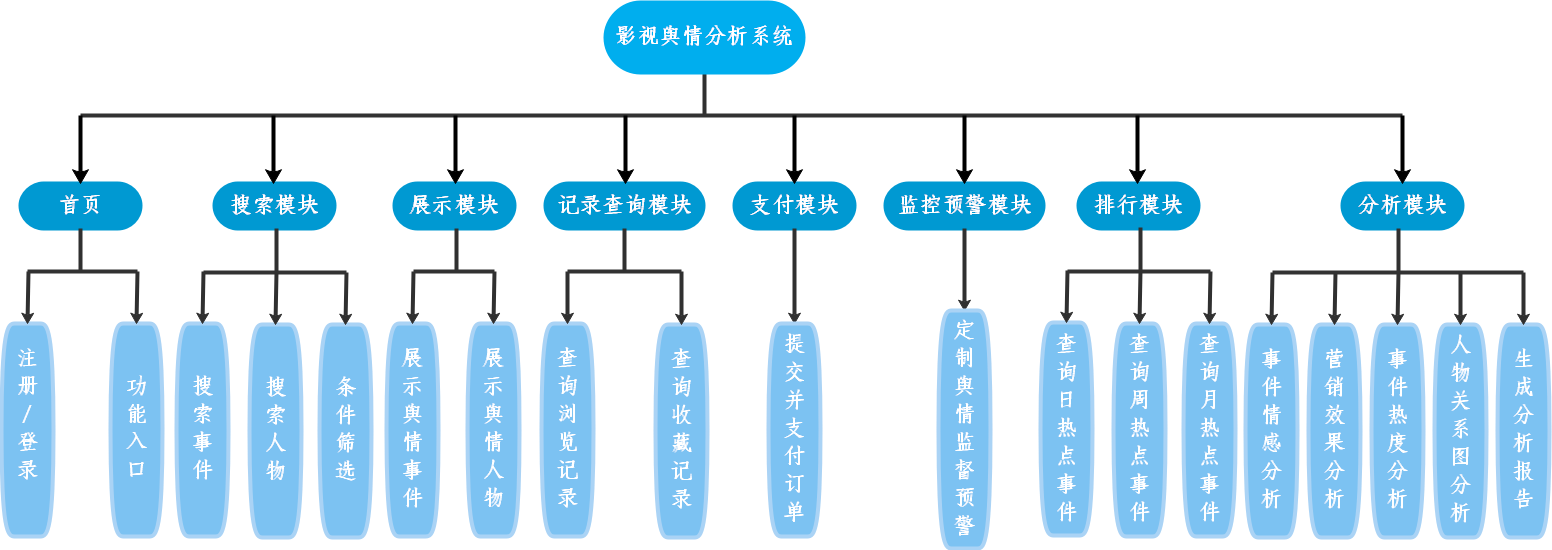
\includegraphics[scale=0.4]{image/o1.png}
	\caption{系统业务层次图}
\end{figure}

\subsubsection{包的设计}
本系统为了能更加有效地进行整合、生产宏观模型,就需要对系统中的类进行分组,以下是本系统中的包设计。本小结以包为单位,对每个包所含有的类及类与类间的调用关系进行说明。
\begin{figure}[!htbp]
	\centering
	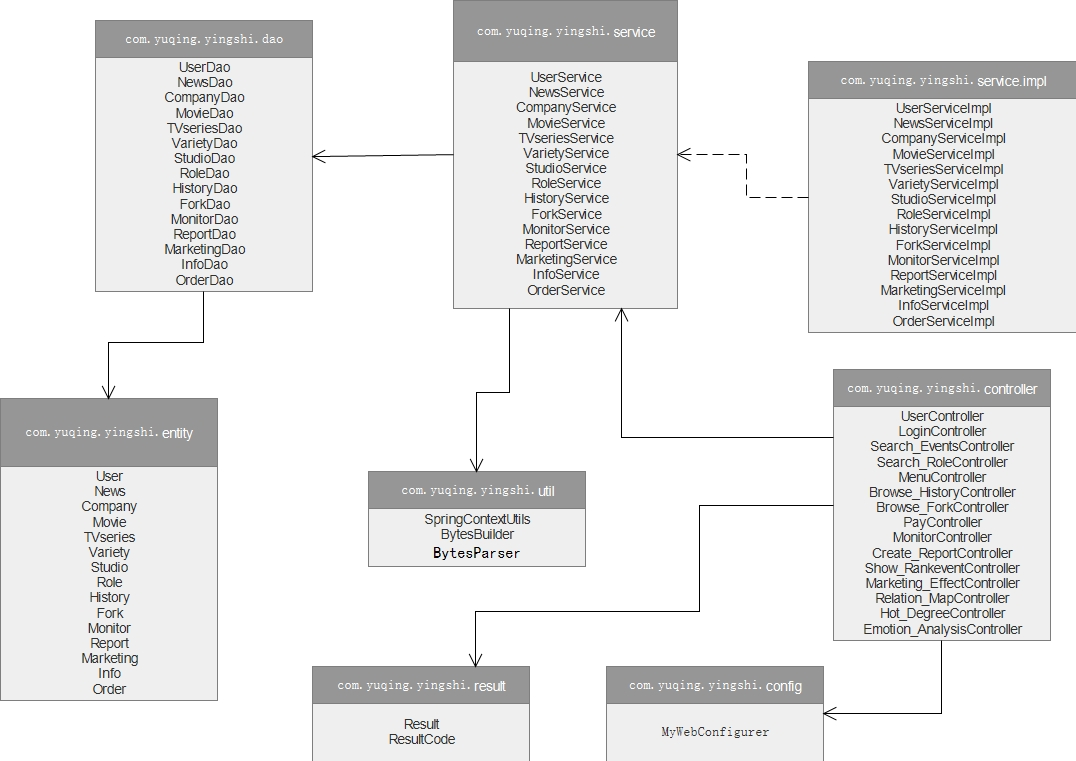
\includegraphics[scale=0.4]{image/o2.png}
	\caption{舆情系统包的设计}
\end{figure}

下表为服务器的包设计表
\begin{tabular}{c c|} 
包名 & 
\multicolumn{2}{c}{设计说明} \\ 
\hline 
com.yuqing.yingshi.service & 该包主要存放了高层调用Dao的接口
com.yuqing.yingshi.controller & 改包主要存放了业务逻辑相关类,依赖于com.yuqing.yingshi.service,调用Service以完成业务逻辑
com.yuqing.yingshi.result& 该包存放了服务器与web端交互时返回的结果对应编码
com.yuqing.yingshi.dao&主要负责数据访问,该包中的类封装了对数据库的访问(只包含最原子的数据操作),供高层调用,依赖于com.yuqing.yingshi.entity
com.yuqing.yingshi.config& 存放了与前端web网页交互的相关配置
com.yuqing.yingshi.entity&该包主要存放数据库表中所对应的实体类
com.yuqing.yingshi.service.impl&该包存放了service包中定义的接口的具体实现
com.yuqing.yingshi.util&存放了项目相关工具类
\end{tabular}


\subsubsection{模块功能介绍}
\begin{itemize}
	\item 注册/登录模块
\end{itemize}
\begin{longtable}[c]{|p{1cm}|p{2cm}|p{10cm}|}
\caption{注册/登录模块功能介绍表}
\label{tab:table1}\\
\hline
\rowcolor[HTML]{DAE8FC} 
序号 & 功能点    & 功能描述                      \\ \hline
\endfirsthead
%
\multicolumn{3}{c}%
{{\bfseries Table \thetable\ continued from previous page}} \\
\endhead
%
1  & 注册     & 用户注册系统,将用户输入信息插入数据库用户表中   \\ \hline
2  & 登录     & 用户登录并可进入个人页面              \\ \hline
3  & 进入功能页面 & 获得授权的用户根据不同的用户类别进入响应的功能界面 \\ \hline
\end{longtable}
\begin{itemize}
	\item 搜索模块
\end{itemize}
\begin{longtable}[c]{|p{1cm}|p{2cm}|p{10cm}|}
	\caption{搜索模块功能介绍表}
	\label{tab:table2}\\
	\hline
	\rowcolor[HTML]{DAE8FC} 
	序号 & 功能点  & 功能描述                      \\ \hline
	\endfirsthead
	%
	\multicolumn{3}{c}%
	{{\bfseries Table \thetable\ continued from previous page}} \\
	\endhead
	%
	1  & 搜索事件 & 用户搜索自己感兴趣的事件,通过关键词来搜索特定事件 \\ \hline
	2  & 搜索人物 & 用户通过输入姓名搜索特定人物            \\ \hline
	3  & 筛选   & 用户通过选择系统提供的关键词筛选人物或事件     \\ \hline
\end{longtable}
\newpage
\begin{itemize}
	\item 展示模块
\end{itemize}
\begin{longtable}[c]{|p{1cm}|p{2cm}|p{10cm}|}
	\caption{展示模块功能介绍表}
	\label{tab:table3}\\
	\hline
	\rowcolor[HTML]{DAE8FC} 
	序号 & 功能点  & 功能描述          \\ \hline
	\endfirsthead
	%
	\multicolumn{3}{c}%
	{{\bfseries Table \thetable\ continued from previous page}} \\
	\endhead
	%
	1  & 展示事件 & 特定展示区域展示推荐的事件 \\ \hline
	2  & 展示人物 & 特定展示区域展示推荐的人物 \\ \hline
\end{longtable}
\begin{itemize}
	\item 记录查询模块
\end{itemize}

\begin{longtable}[c]{|p{1cm}|p{3cm}|p{9cm}|}
	\caption{记录查询模块功能介绍表}
	\label{tab:table3}\\
	\hline
	\rowcolor[HTML]{DAE8FC} 
	序号 & 功能点    & 功能描述              \\ \hline
	\endfirsthead
	%
	\multicolumn{3}{c}%
	{{\bfseries Table \thetable\ continued from previous page}} \\
	\endhead
	%
	1  & 查询浏览记录 & 用户查询近期内浏览的舆情事件和人物 \\ \hline
	2  & 查询收藏记录 & 用户查询自己的收藏记录       \\ \hline
\end{longtable}
\begin{itemize}
	\item 支付模块
\end{itemize}
\begin{longtable}[c]{|p{1cm}|p{2cm}|p{10cm}|}
	\caption{支付模块功能介绍表}
	\label{tab:table4}\\
	\hline
	\rowcolor[HTML]{DAE8FC} 
	序号 & 功能点  & 功能描述                   \\ \hline
	\endfirsthead
	%
	\multicolumn{3}{c}%
	{{\bfseries Table \thetable\ continued from previous page}} \\
	\endhead
	%
	1  & 支付订单 & 用户提交订单后按照流程完成支付,获得系统授权 \\ \hline
\end{longtable}
\begin{itemize}
	\item 监控预警模块
\end{itemize}

\begin{longtable}[c]{|p{1cm}|p{2cm}|p{10cm}|}
	\caption{监控预警模块功能介绍表}
	\label{tab:table5}\\
	\hline
	\rowcolor[HTML]{DAE8FC} 
	序号 & 功能点      & 功能描述                            \\ \hline
	\endfirsthead
	%
	\multicolumn{3}{c}%
	{{\bfseries Table \thetable\ continued from previous page}} \\
	\endhead
	%
	1  & 定制舆情监控预警 & 企业用户可以对某一舆情事件定制监控预警,以便及时对事件作出回应 \\ \hline
\end{longtable}
\newpage
\begin{itemize}
	\item 排行模块
\end{itemize}
\begin{longtable}[c]{|p{1cm}|p{2cm}|p{10cm}|}
	\caption{排行模块功能介绍表}
	\label{tab:table6}\\
	\hline
	\rowcolor[HTML]{DAE8FC} 
	序号 & 功能点    & 功能描述                         \\ \hline
	\endfirsthead
	%
	\multicolumn{3}{c}%
	{{\bfseries Table \thetable\ continued from previous page}} \\
	\endhead
	%
	1  & 查询日排行榜 & 用户选取时间区间为单日并可查看单日热点影视舆情事件排行榜 \\ \hline
	2  & 查询周排行榜 & 用户选取时间区间为一周并可查看本周热点影视舆情事件排行榜 \\ \hline
	3  & 查询月排行榜 & 用户选取时间区间为一月并可查看本月热点影视舆情事件排行榜 \\ \hline
\end{longtable}
\begin{itemize}
	\item 分析模块
\end{itemize}

\begin{longtable}[c]{|p{1cm}|p{3cm}|p{9cm}|}
	\caption{分析模块功能介绍表}
	\label{tab:table7}\\
	\hline
	\rowcolor[HTML]{DAE8FC} 
	序号 & 功能点    & 功能描述                            \\ \hline
	\endfirsthead
	%
	\multicolumn{3}{c}%
	{{\bfseries Table \thetable\ continued from previous page}} \\
	\endhead
	%
	1  & 情感分析   & 系统根据算法对影视舆情事件进行情感分析,绘制时间-情感图    \\ \hline
	2  & 热度分析   & 对特定舆情事件在不同平台的热度(包括访问、转发等)进行统计分析 \\ \hline
	3  & 营销效果分析 & 通过系统设定的指标,对企业用户设定的营销事件进行营销效果分析  \\ \hline
	4  & 人物关系分析 & 对影视舆情人物以事件为关系生成人物关系图谱           \\ \hline
	5  & 生成分析报告 & 根据特定的事件系统生成舆情分析报告               \\ \hline
\end{longtable}
\subsubsection{模块间接口设计}
